\chapter{图表及公式的格式说明}
\echapter{figure and table}%
\label{cha:figure_and_table}



\section{图的格式说明}
\esection{format of figure}%
\label{sec:format_of_figure}

\begin{figure}[htpb]
    \centering
    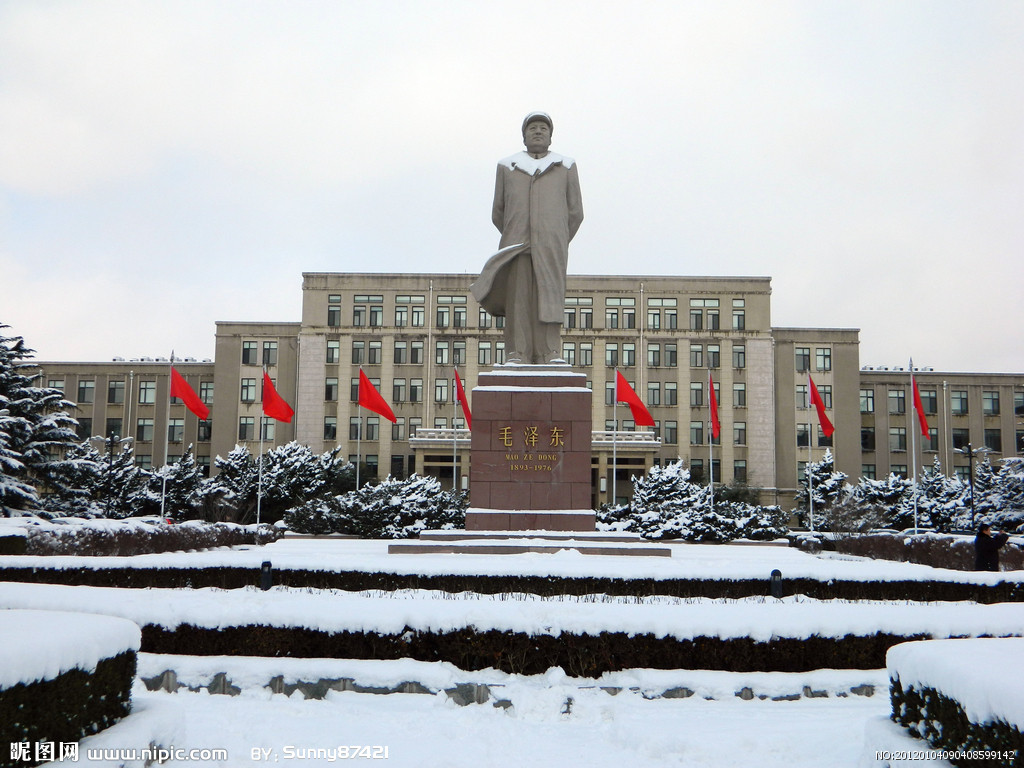
\includegraphics[width=0.8\linewidth]{figures/cmm.jpg}
    \bicaption[fig:cmm]{毛主席雕像}{毛主席像,请问主席举起哪一只手。}{Fig.}{Which hand of chirman Miao is up}
\end{figure}
表、图序号后面,同样适当留空(汉字状态敲两次空格键)。

图\ref{fig:cmm}显示了论文模板中所定义的样式选择方法。使用鼠标选择相应的样式,对应的文字格式就发生相应改变

\section{ 图的格式描述}
\esection{describe of figure format}
\begin{enumerate}[(1)]
\item 图的绘制方法
    \begin{asparaenum}[1)]
    \item 插图、照片应尽量通过扫描粘贴进本文。

    \item 简单文字图可用WORD直接绘制。
    \end{asparaenum}
\item 图的位置
    \begin{asparaenum}[1)]
    \item  图居中排列。

    \item 图与上文之间应留一空行。

    \item 图中若有附注,一律用阿拉伯数字和右半圆括号按顺序编排,如注1),附注写在图的下方。
    \end{asparaenum}
\item 图的版式
    \begin{asparaenum}[1)]
    \item “设置图片格式”的“版式”为“上下型”或“嵌入型”,不得“浮于文字之上”。

    \item 图的大小尽量以一页的页面为限,不要超限,一旦超限要加续图。
    \end{asparaenum}
\item 图名的写法
    \begin{asparaenum}[1)]
    \item 图名居中并位于图下,编号应分章编号,如图3.1。

    \item 图名与下文留一空行。

    \item 图及其名称要放在同一页中,不能跨接两页。

    \item 图内文字清晰、美观。

    \item 中文图名设置为黑体,小四号,居中。英文名称设置为Times New Roman,小四号,居中。 
    \end{asparaenum}
\end{enumerate}

\subsection{表的格式说明}
\esubsection{format of table}

\subsection{表格的格式示例}
\esubsection{example of table format}

表在正文中的常用格式如表3.1-3.3所示,使用三线表。

物流的概念和范围如表3.1表述。

表、图序号与后面文字同样应当适当留空(两次空格键)。
\begin{table}[h]
    \bicaption[tab:chap02:logistics]{物流的概念和范围}{物流的概念和范围}{Tab.}{Conception and scope of Logistics}
    \centering
    \vspace{0.2cm}
    \wuhao
    \begin{tabular}{cc}
    \hline
    {\hei 本质} & {\hei 过程}\\
    \hline
    途径或方法 & 规划、实施、控制\\
    目标 & {效率、成本效益}\\
    活动或作业 & 流动与储存\\
    处理对象 & 原材料、在制品、产成品、相关信息\\
    范围 & 从原点(供应商)到终点(最终顾客)\\
    目的或目标 & 适应顾客的需求(产品、功能、数量、质量、时间、价格)\\
    \hline
    \end{tabular}
\end{table}

美国广义物流后(勤)协会给出的定义如下:“为了符合顾客的要求,
从原点到消费点对原材料、在制品、产成品与相关信息的流动和
储存的效率成本效益进行规划、实施和控制的过程”。由此可见,
物流不是作为一种具体技术和方法来研究的,而是一个过程或管理。

\subsection{表的格式描述}
\esubsection{describe of table format}
\begin{enumerate}[(1)]
    \item  表的绘制方法

表要用WORD绘制,不要粘贴。如果要求使用Excel表格,则使用数值粘贴。
    \item   表的位置
	\begin{asparaenum}[1)]
       \item  表格居中排列。

       \item 表格与下文应留一行空格。

       \item 表中若有附注,一律用阿拉伯数字和右半圆括号按顺序编排,如注1),附注写在表的下方。
       \end{asparaenum}
    \item 表的版式
	\begin{asparaenum}[1)]
	\item 表的大小尽量以一页的页面为限,不要超限,一旦超限要加续表。
	\end{asparaenum}
    \item 表名的写法
    \begin{asparaenum}[1)]
	\item 表名应当在表的上方并且居中。编号应分章编号,如表3.1、表3.2。

	\item 表名与上文留一空行。

	\item 表及其名称要放在同一页中,不能跨接两页。

	\item 表内文字全文统一,设置为宋体,五号。

	\item 中文表名设置为宋体,小四号,且居中。英文名称设置为Times New Roman,小四号,且居中。
    \end{asparaenum}

\end{enumerate}

\section{公式的格式说明}
\esection{formula format}%
\label{sec:formula_format}
\subsection{公式格式示例}
\esubsection{example for formula}
由于一般的文献资料中所给出的载荷和抗力的统计参数主要为变异系数,为便于讨论,定义公式形式如下:
\begin{equation}
    \textrm{LRI} = 1  \bigg / \sqrt{1 + \qty (\frac{\mu_R}{\mu_s})^2 \qty (\frac{\delta_R}{\delta_S})^2 }
    \label{Eq:31}
\end{equation}
其中,$\mu_R, \mu_S$分别为抗力和载荷的均值\dots 。

\subsection{公式的格式描述}
\esubsection{describe of math format}

\begin{asparaenum}[(1)]
\item 公式整行右对齐,并调整公式与公式序号之间的距离,使公式部分居中显示。

\item 公式序号应按章编号,公式编号在行末列出,如 \eqref{Eq:31}。

\item 公式位置:公式之间及上下文间设置半行间距或者6磅,作者可根据情况适当调整,以保证格式协调和美观。
\end{asparaenum}

\section{参考文献的格式说明}
\esection{explain of format of reference}

\subsection{参考文献在正文中引用的示例}
\esubsection{example for citation}
大连理工大学的量子力学课程使用宋鹤山老师的教材\cite{BOOK.hssong2006},
也可以参考张永德老师的高等量子力学教材\cite{BOOK.Zhang2009}
